% A CONSORT-style flowchart of a randomized controlled trial
% using the PGF/TikZ package
% Author  : Morten Vejs Willert (July 2010)
% License : Creative Commons attribution license
\documentclass[10pt]{article}
\usepackage[latin1]{inputenc}
\usepackage[left=0.2in,right=0.2in,top=0.25in,bottom=0.2in]{geometry}
\usepackage{tikz}
\usetikzlibrary{positioning,shapes,arrows,fit,calc}
\usepackage{caption}
\usepackage{amsmath}
\usepackage{verbatimbox}
\usepackage[framed]{matlab-prettifier}
\usepackage{filecontents}
\usepackage[scaled]{helvet}
\usepackage[bitstream-charter]{mathdesign}
%\usepackage{XCharter}
\renewcommand\familydefault{\sfdefault}
\usepackage[scaled]{beramono}
\usepackage[T1]{fontenc}
\usepackage{multicol}
\usepackage{xcolor}
\definecolor{oblue}{rgb}{0.4745,0.6,0.8}
\colorlet{dblue}{oblue!80!black}
\usepackage{enumitem}
\setitemize{noitemsep,topsep=0pt,parsep=0pt,partopsep=0pt}

% newcommand{\tikzmark}[1]{\tikz[overlay,remember picture] \node (#1) {};}

% \tikzset{
%  font={\fontsize{10pt}{12}\selectfont}}

%  \vfill\null
%\columnbreak

% TODO rounded code block frames does not work with a background color
% (background color spills out of the rounded corner).
\lstset{
%frameround=tttt,
backgroundcolor=\color{oblue!10!white}
}

	\tikzstyle{object} = [draw=oblue, very thick,
    	rectangle, rounded corners, inner sep=7pt]
\begin{document}
\begin{center}

{\large\textbf{OpenSim Moco Cheat Sheet for the Matlab Interface}}

  \begin{tikzpicture}[auto]
    

    
\node (studybody) [align=left, text width=7in] {
\vspace{-15pt}
\begin{center}\textbf{\textcolor{oblue}{MocoStudy}}\end{center}
};
    
    \node (problem) at ([shift={(270:5.3)}]studybody.south) [object, dash pattern=on 10pt off 1pt, align=left, text width=7.5in] {
\vspace{-10pt}
\begin{center}\textbf{\textcolor{oblue}{MocoProblem}}\end{center}
\begin{multicols}{2}% 2-column layout
Access the MocoProblem from the study.
\begin{lstlisting}[style=Matlab-editor, basicstyle=\mlttfamily\small, linewidth=0.48\textwidth]
problem = study.updProblem();
\end{lstlisting}
\vspace{5pt}
\textbf{Set the model.}\\
\begin{lstlisting}[style=Matlab-editor, basicstyle=\mlttfamily\small, linewidth=0.48\textwidth]
problem.setModel(Model('model_file.osim'));
\end{lstlisting}
\vspace{5pt}
\textbf{Set variable bounds.}\\
Set initial time to 0; final time between 0.5 and 1.5 s.
\begin{lstlisting}[style=Matlab-editor, basicstyle=\mlttfamily\small, linewidth=0.48\textwidth]
problem.setTimeBounds(MocoInitialBounds(0), MocoFinalBounds(0.5, 1.5));
\end{lstlisting}
The coordinate value must be between 0 and $\pi$ over the phase, 
and its initial value is 0 and its final value is $\pi/2$.
\begin{lstlisting}[style=Matlab-editor, basicstyle=\mlttfamily\small, linewidth=0.48\textwidth]
problem.setStateInfo('/jointset/j0/q0/value', 
    [0, pi], 0, pi/2);
\end{lstlisting}
The control for actuator `/tau0' must be within [-50, 50] over the phase.
\begin{lstlisting}[style=Matlab-editor, basicstyle=\mlttfamily\small, linewidth=0.48\textwidth]
problem.setControlInfo('/tau0', [-50, 50]);
\end{lstlisting}
  \vfill\null
\columnbreak
\textbf{Optimize static model properties.}\\
Create parameter `myparam' to optimize the mass of Body `/bodyset/b0' within [0.1, 0.5].
\begin{lstlisting}[style=Matlab-editor, basicstyle=\mlttfamily\small, linewidth=0.48\textwidth]
problem.addParameter(MocoParameter('myparam',
    '/bodyset/b0', 'mass', MocoBounds(0.1, 0.5)));
\end{lstlisting}
\vspace{5pt}
\textbf{Add goals to the problem.}
\begin{center}
Control $\cdot $ ControlTracking $\cdot$ FinalTime \\
StateTracking $\cdot$ MarkerTracking $\cdot$ TranslationTracking \\
OrientationTracking $\cdot$ JointReaction
\end{center}
Minimize the sum of squared controls with weight 1.5.
\begin{lstlisting}[style=Matlab-editor, basicstyle=\mlttfamily\small, linewidth=0.48\textwidth]
problem.addGoal(MocoControlGoal('effort', 1.5));    
\end{lstlisting}
\vspace{5pt}
\textbf{Add path constraints to the problem.}\\
Define time-dependent bounds for controls.
\begin{lstlisting}[style=Matlab-editor, basicstyle=\mlttfamily\small, linewidth=0.48\textwidth]
pathCon = MocoControlBoundConstraint();
problem.addPathConstraint(pathCon);
\end{lstlisting}
\end{multicols}
};
    
\node (solver) at ([shift={(270:5.8)}]problem.south) [object,  dash pattern=on 10pt off 1pt, align=left, text width=7.5in] {
\vspace{-10pt}
\begin{center}\textbf{\textcolor{oblue}{MocoSolver}}\end{center}
\begin{multicols}{2}% 2-column layout
\textbf{Initialize the CasADi or Tropter solver.}\\
\begin{lstlisting}[style=Matlab-editor, basicstyle=\mlttfamily\small, linewidth=0.48\textwidth]
solver = study.initCasADiSolver();
% alternative: solver = study.initTropterSolver();
\end{lstlisting}
\vspace{5pt}
\textbf{Settings for Tropter and CasADi solvers.}\\
Solve the problem on a grid of 51 mesh points.
\begin{lstlisting}[style=Matlab-editor, basicstyle=\mlttfamily\small, linewidth=0.48\textwidth]
solver.set_num_mesh_intervals(50);
\end{lstlisting}
Transcribe the optimal control problem with the Hermite-Simpson scheme (alternative: `trapezoidal').
\begin{lstlisting}[style=Matlab-editor, basicstyle=\mlttfamily\small, linewidth=0.48\textwidth]
solver.set_transcription_scheme('hermite-simpson');
\end{lstlisting}
Loosen the convergence and constraint tolerances.
\begin{lstlisting}[style=Matlab-editor, basicstyle=\mlttfamily\small, linewidth=0.48\textwidth]
solver.set_convergence_tolerance(1e-3);
solver.set_constraint_tolerance(1e-3);
\end{lstlisting}
Stop optimization after 500 iterations.
\begin{lstlisting}[style=Matlab-editor, basicstyle=\mlttfamily\small, linewidth=0.48\textwidth]
solver.set_max_iterations(500);
\end{lstlisting}
By default, the Hessian is approximated from first derivatives. Set to 'exact' to use an exact Hessian.
\begin{lstlisting}[style=Matlab-editor, basicstyle=\mlttfamily\small, linewidth=0.48\textwidth]
solver.set_optim_hessian_approximation('exact');
\end{lstlisting}
\columnbreak
Create a guess, randomize it, then set the guess.
\begin{lstlisting}[style=Matlab-editor, basicstyle=\mlttfamily\small, linewidth=0.48\textwidth]
guess = solver.createGuess(); guess.randomizeAdd();
solver.setGuess(guess);
\end{lstlisting}
Set the guess from a MocoTrajectory or MocoSolution file.
\begin{lstlisting}[style=Matlab-editor, basicstyle=\mlttfamily\small, linewidth=0.48\textwidth]
solver.setGuessFile('previous_solution.sto');
\end{lstlisting}

\vspace{5pt}
\textbf{Settings for only CasADi solver.}\\
By default, CasADi uses 'central' finite differences; 'forward' differences are faster but less accurate.
\begin{lstlisting}[style=Matlab-editor, basicstyle=\mlttfamily\small, linewidth=0.48\textwidth]
solver.set_finite_difference_scheme('forward');
\end{lstlisting}
Turn off parallel calculations.
\begin{lstlisting}[style=Matlab-editor, basicstyle=\mlttfamily\small, linewidth=0.48\textwidth]
solver.set_parallel(0);
\end{lstlisting}
Monitor solver progress by writing every 10th iterate to file.
\begin{lstlisting}[style=Matlab-editor, basicstyle=\mlttfamily\small, linewidth=0.48\textwidth]
solver.set_output_interval(10);
\end{lstlisting}
\end{multicols}
};

\node (studypost) at ([shift={(270:1.3)}]solver.south) [align=left, text width=7.5in] {
\begin{multicols}{2}% 2-column layout
    
Solve the study and obtain a MocoSolution.
\begin{lstlisting}[style=Matlab-editor, basicstyle=\mlttfamily\small, linewidth=0.48\textwidth]
solution = study.solve();
\end{lstlisting}
Visualize the solution.
\begin{lstlisting}[style=Matlab-editor, basicstyle=\mlttfamily\small, linewidth=0.48\textwidth]
study.visualize(solution);
\end{lstlisting}
Compute outputs from the solution.
\begin{lstlisting}[style=Matlab-editor, basicstyle=\mlttfamily\small, linewidth=0.48\textwidth]
outputs = StdVectorString();
outputs.add('.*active_force_length_multiplier');
table = study.analyze(solution, outputs);
\end{lstlisting}
\end{multicols}
};
    
    
    \node (study) [object, fit={(studybody) (problem) (solver) (studypost)}] {};
  \end{tikzpicture}
\end{center}
    
    \newpage
    
    
    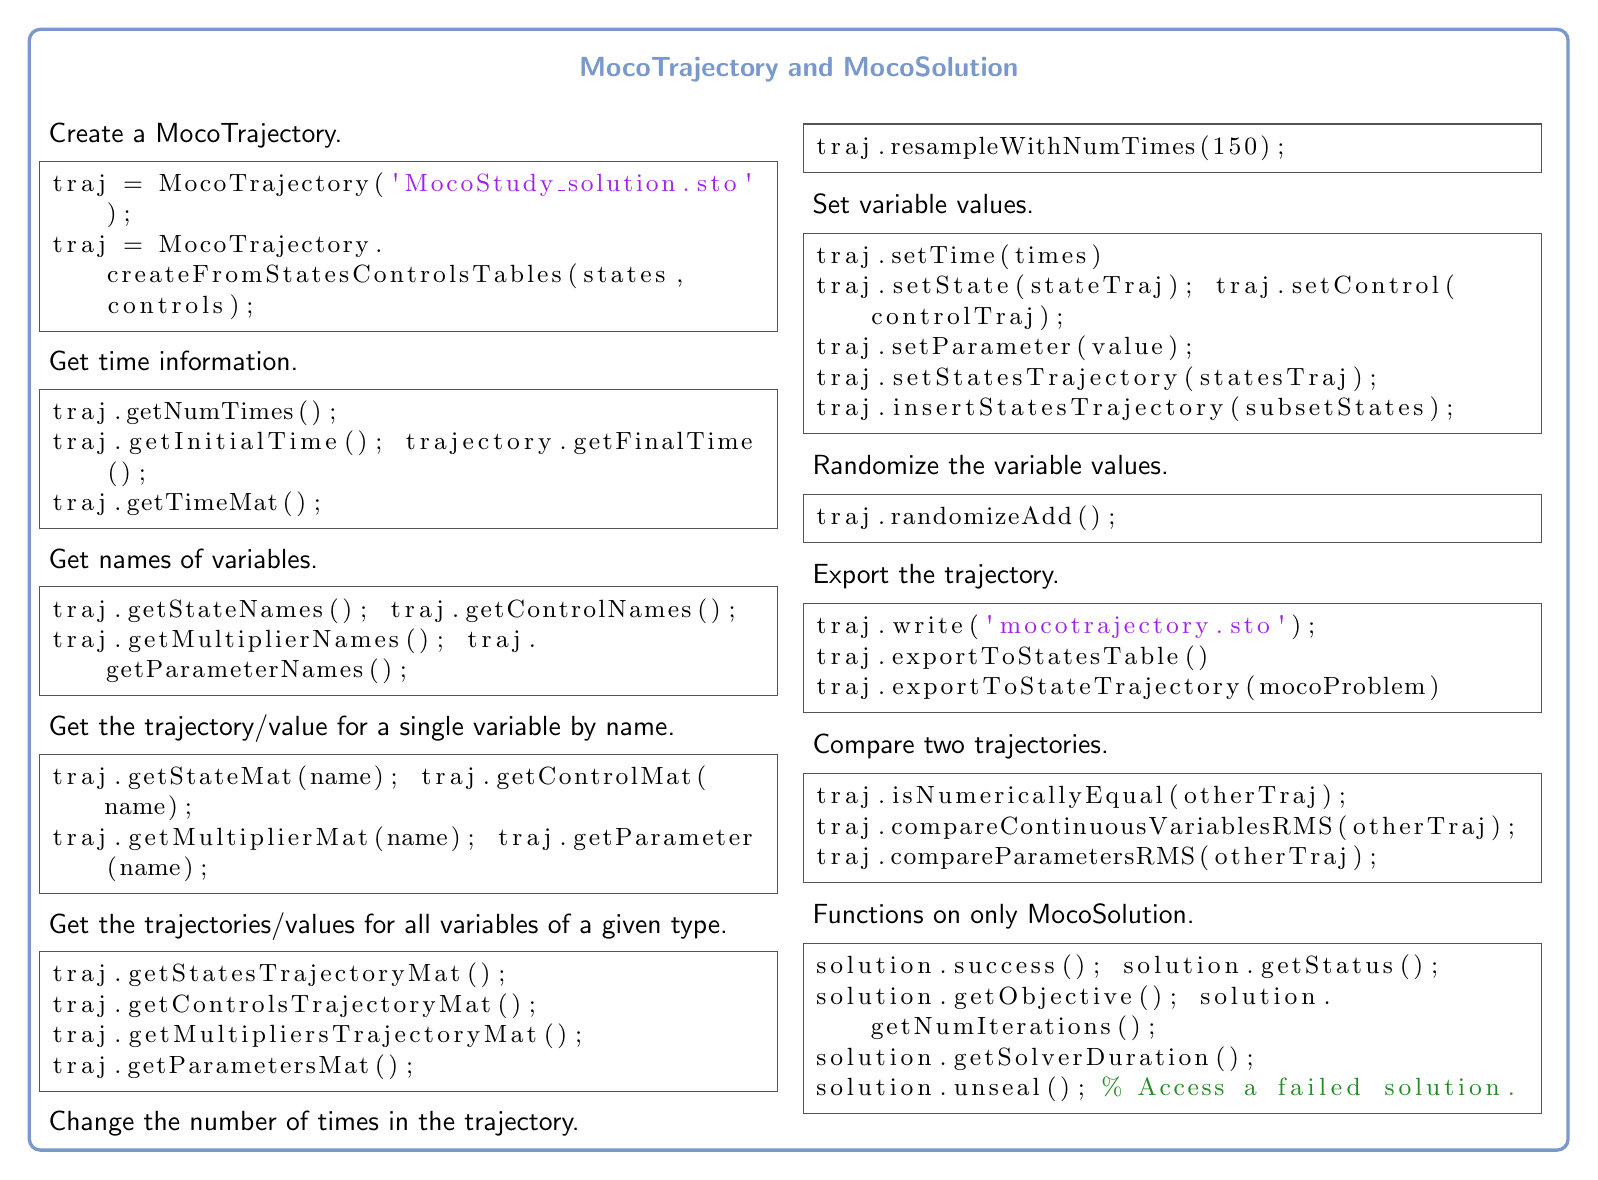
\begin{tikzpicture}[auto]
    \node (trajectory) [object, align=left, text width=7.5in] {
\vspace{-10pt}
\begin{center}\textbf{\textcolor{oblue}{MocoTrajectory and MocoSolution}}\end{center}
\vspace{-15pt}
\begin{multicols}{2}% 2-column layout
Create a MocoTrajectory.
\begin{lstlisting}[style=Matlab-editor, basicstyle=\mlttfamily\small, linewidth=0.48\textwidth]
traj = MocoTrajectory('MocoStudy_solution.sto');
traj = MocoTrajectory.createFromStatesControlsTables(states, controls);
\end{lstlisting}
Get time information.
\begin{lstlisting}[style=Matlab-editor, basicstyle=\mlttfamily\small, linewidth=0.48\textwidth]
traj.getNumTimes();
traj.getInitialTime(); trajectory.getFinalTime();
traj.getTimeMat();
\end{lstlisting}
Get names of variables.
\begin{lstlisting}[style=Matlab-editor, basicstyle=\mlttfamily\small, linewidth=0.48\textwidth]
traj.getStateNames(); traj.getControlNames();
traj.getMultiplierNames(); traj.getParameterNames();
\end{lstlisting}
Get the trajectory/value for a single variable by name.
\begin{lstlisting}[style=Matlab-editor, basicstyle=\mlttfamily\small, linewidth=0.48\textwidth]
traj.getStateMat(name); traj.getControlMat(name);
traj.getMultiplierMat(name); traj.getParameter(name);
\end{lstlisting}
Get the trajectories/values for all variables of a given type.
\begin{lstlisting}[style=Matlab-editor, basicstyle=\mlttfamily\small, linewidth=0.48\textwidth]
traj.getStatesTrajectoryMat();
traj.getControlsTrajectoryMat();
traj.getMultipliersTrajectoryMat();
traj.getParametersMat();
\end{lstlisting}

Change the number of times in the trajectory.
\begin{lstlisting}[style=Matlab-editor, basicstyle=\mlttfamily\small, linewidth=0.48\textwidth]
traj.resampleWithNumTimes(150);
\end{lstlisting}
Set variable values.
\begin{lstlisting}[style=Matlab-editor, basicstyle=\mlttfamily\small, linewidth=0.48\textwidth]
traj.setTime(times)
traj.setState(stateTraj); traj.setControl(controlTraj);
traj.setParameter(value);
traj.setStatesTrajectory(statesTraj);
traj.insertStatesTrajectory(subsetStates);
\end{lstlisting}
Randomize the variable values.
\begin{lstlisting}[style=Matlab-editor, basicstyle=\mlttfamily\small, linewidth=0.48\textwidth]
traj.randomizeAdd();
\end{lstlisting}
Export the trajectory.
\begin{lstlisting}[style=Matlab-editor, basicstyle=\mlttfamily\small, linewidth=0.48\textwidth]
traj.write('mocotrajectory.sto');
traj.exportToStatesTable()
traj.exportToStateTrajectory(mocoProblem)
\end{lstlisting}
Compare two trajectories.
\begin{lstlisting}[style=Matlab-editor, basicstyle=\mlttfamily\small, linewidth=0.48\textwidth]
traj.isNumericallyEqual(otherTraj);
traj.compareContinuousVariablesRMS(otherTraj);
traj.compareParametersRMS(otherTraj);
\end{lstlisting}
Functions on only MocoSolution.
\begin{lstlisting}[style=Matlab-editor, basicstyle=\mlttfamily\small, linewidth=0.48\textwidth]
solution.success(); solution.getStatus();
solution.getObjective(); solution.getNumIterations();
solution.getSolverDuration();
solution.unseal(); % Access a failed solution.
\end{lstlisting}
\end{multicols}
};    
    \end{tikzpicture}
    
    
% TODO put in a tikz box.
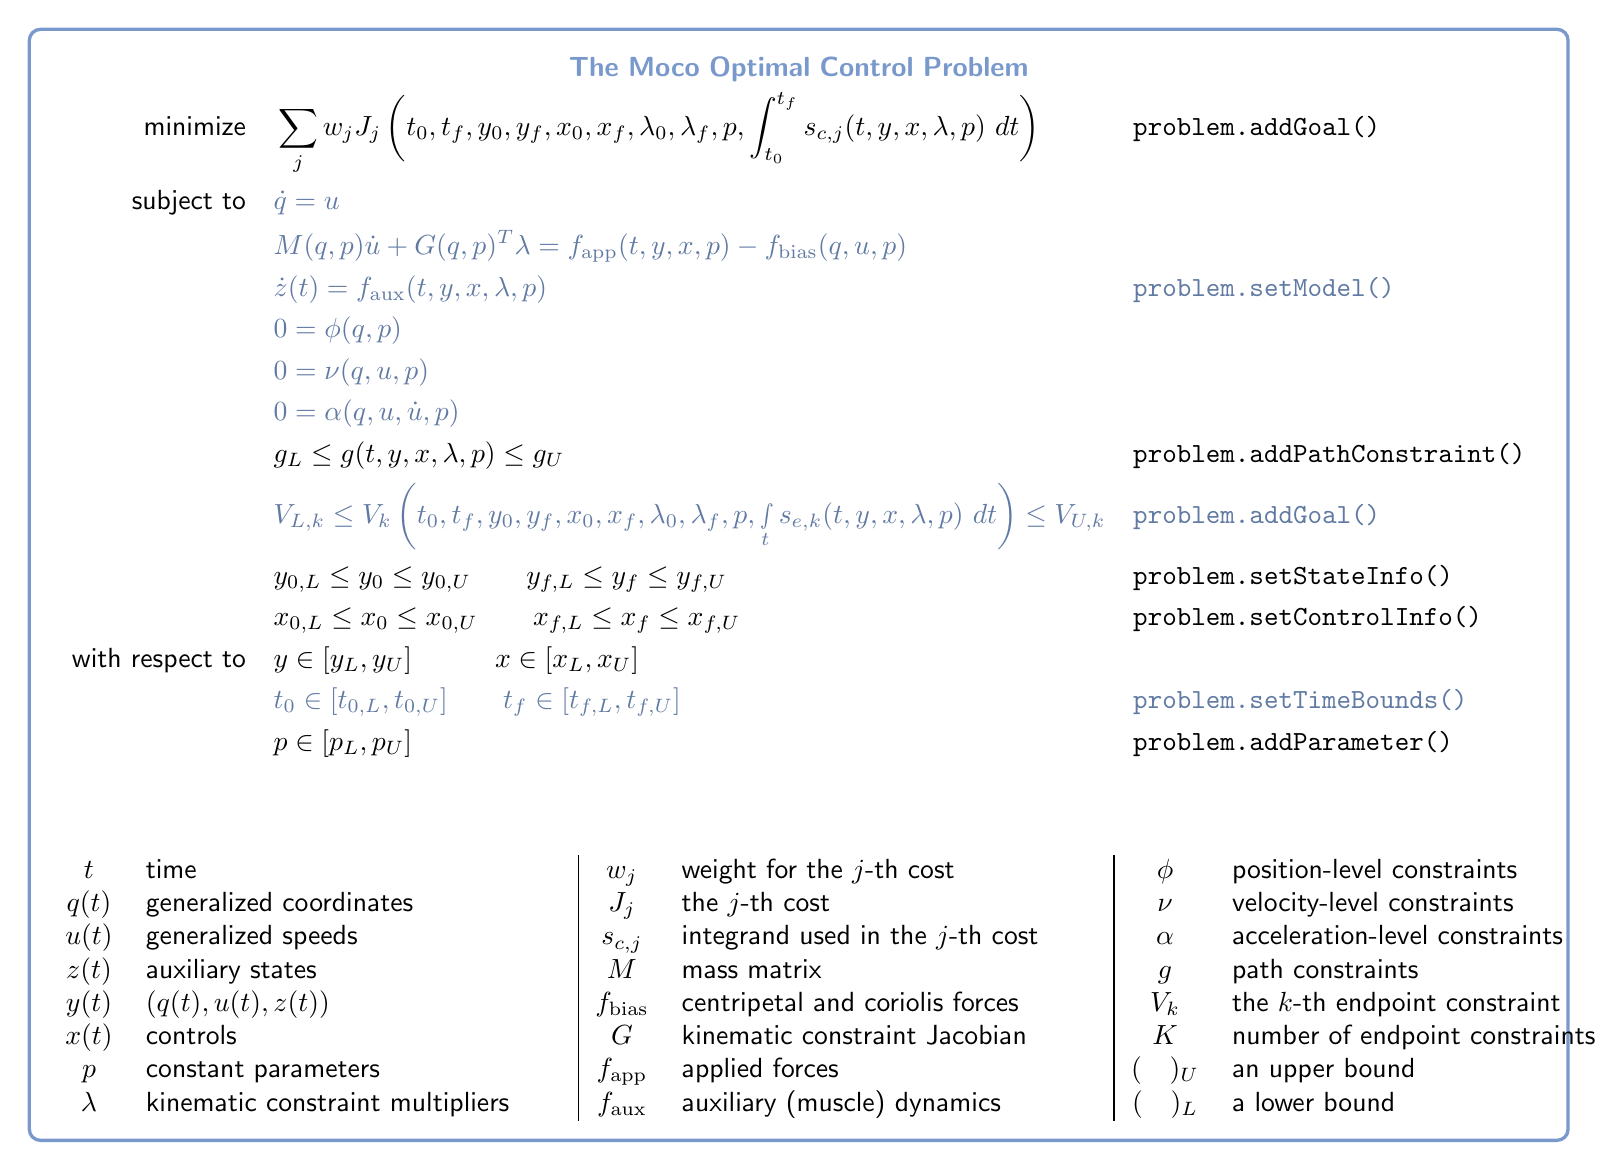
\begin{tikzpicture}
\node (ocp) [object, align=left, text width=7.5in] {
\vspace{-10pt}
\begin{center}\textbf{\textcolor{oblue}{The Moco Optimal Control Problem}}\end{center}
\vspace{-15pt}
    \begin{align*}
        \mbox{minimize}
         \quad & \sum_j w_{j} J_{j}\displaystyle\left(t_0, t_f, y_0, y_f, x_{0}, x_{f}, \lambda_0, \lambda_f, p, \int_{t_0}^{t_f} s_{c,j}(t, y, x, \lambda, p)~dt \displaystyle\right) && \texttt{problem.addGoal()}   \\
        \mbox{subject to}
         \quad & \textcolor{dblue}{\dot{q} = u} && \\
         & \textcolor{dblue}{M(q, p)\dot{u} + G(q, p)^T \lambda = f_{\textrm{app}}(t, y, x, p) - f_{\textrm{bias}}(q, u, p)} \\
         & \textcolor{dblue}{\dot{z}(t) = f_{\textrm{aux}}(t, y, x, \lambda, p)} &&\texttt{\textcolor{dblue}{problem.setModel()}} \\
         & \textcolor{dblue}{0 = \phi(q, p)} \\
         & \textcolor{dblue}{0 = \nu(q, u, p)} \\
         &  \textcolor{dblue}{0 = \alpha(q, u, \dot{u}, p)} \\
         & g_{L} \leq g(t, y, x, \lambda, p) \leq g_{U} && \texttt{problem.addPathConstraint()} \\
         & \textcolor{dblue}{V_{L,k} \leq V_{k}\displaystyle\left(t_0,t_f,y_0, y_f, x_0, x_f, \lambda_0, \lambda_f, p, \smallint_{t} s_{e,k}(t,y,x,\lambda,p)~dt\displaystyle\right) \leq V_{U,k}} && \texttt{\textcolor{dblue}{problem.addGoal()}} \\
         & {y_{0,L} \leq y_0 \leq y_{0,U} \quad\quad y_{f,L} \leq y_f \leq y_{f,U}} && \texttt{problem.setStateInfo()} \\
         & {x_{0,L} \leq x_0 \leq x_{0,U} \quad\quad x_{f,L} \leq x_f \leq x_{f,U}} && \texttt{{problem.setControlInfo()}} \\
         \mbox{with respect to} \quad
         & {y \in [y_{L}, y_{U}] \quad\quad\quad x \in [x_{L}, x_{U}]} \\
         & \textcolor{dblue}{t_0 \in [t_{0,L}, t_{0,U}] \quad\quad  t_f \in [t_{f,L}, t_{f,U}]} && \texttt{\textcolor{dblue}{problem.setTimeBounds()}} \\
         & {p \in [p_{L}, p_{U}]} && \texttt{{problem.addParameter()}} \\
    \end{align*}

\begin{center}
    \begin{tabular}{cp{15em}|cp{15em}|cp{15em}}
    $ t    $     & time                                                 & $ w_j $               & weight for the $j$-th cost              & $ \phi $                     & position-level constraints \\
    $ q(t) $     & generalized coordinates                              & $ J_j $               & the $j$-th cost                         & $ \nu    $                   & velocity-level constraints \\
    $ u(t) $     & generalized speeds                                   & $ s_{c,j} $           & integrand used in the $j$-th cost       & $ \alpha    $                & acceleration-level constraints\\
    $ z(t) $     & auxiliary states                                     & $ M $                 & mass matrix                             & $ g $                        & path constraints \\
    $ y(t) $     & $ (q(t),u(t),z(t)) $                                 & $ f_{\textrm{bias}} $ & centripetal and coriolis forces         & $ V_k $                      & the $k$-th endpoint constraint \\
    $ x(t) $     & controls                                             & $ G $                 & kinematic constraint Jacobian           & $ K $                        & number of endpoint constraints \\
    $ p    $     & constant parameters                                  & $ f_{\textrm{app}} $  & applied forces                          & $ (\hspace{1em})_{U}   $     & an upper bound \\
    $ \lambda $  & kinematic constraint multipliers                     & $ f_{\textrm{aux}} $  & auxiliary (muscle) dynamics             & $ (\hspace{1em})_{L}   $     & a lower bound \\
\end{tabular}
\end{center}

};
\end{tikzpicture}


\end{document}

% TODO
% add equations to the back side
% add MocoTrajectory interface
% add generic functions in MocoStudy.
% solve()
% visualize()
% analyze()
% add Utilities

%    block_center/.style ={
%    	rectangle, rounded corners,
%    	draw=black, very thick,
%      	text width=8em, text centered,
%      	minimum height=4em,
%      	inner sep=10pt,
%      	inner ysep=10pt,
%      	% minimum width=50em,
%      },
%    block_left/.style ={
%    	rectangle, rounded corners,
%    	draw=black, very thick,
%      	text width=8em,
%      	minimum height=4em,
%      	inner sep=10pt,
%      	inner ysep=10pt,
%      	minimum width=50em
%      	},
%    block_noborder/.style ={rectangle, draw=none, thick, fill=none,
%      text width=18em, text centered, minimum height=1em},
%    block_assign/.style ={rectangle, draw=black, thick, fill=white,
%      text width=18em, text ragged, minimum height=3em, inner sep=6pt},
%    block_lost/.style ={rectangle, draw=black, thick, fill=white,
%      text width=16em, text ragged, minimum height=3em, inner sep=6pt},
%      line/.style ={draw, thick, -latex', shorten >=0pt}]
%
%
